\chapter{Chebyshev polynomials}%
\label{cha:Chebyshev polynomials}

The Chebyshev polynomials $(T_n)_{n \in \nat}$ are given on $[-1, 1]$ by the formula
\begin{equation}
    \label{eq:chebyshev}
    \forall x \in [-1, 1], \qquad
    T_n(x) = \cos \bigl(n \arccos(x)\bigr).
\end{equation}
Although this formula makes sense only if $x \in [-1, 1]$,
the polynomials are defined for all $x \in \real$.
Equivalently,
the Chebyshev polynomials can be defined from
\begin{equation}
    \label{eq:chebyshev_cosh}
    \forall x \in [1, \infty), \qquad
    T_n(x) = \cosh \bigl(n \arccosh(x)\bigr).
\end{equation}
where $\cosh(\theta) = \frac{1}{2} \left( \e^\theta + \e^{-\theta} \right)$ and $\arccosh = \cosh^{-1}(\theta)$ is the inverse function
with codomain~$[0, \infty)$,
so that the inverse is uniquely defined.
The first few Chebyshev polynomials are illustrated in~\cref{fig:chebyshev}.

\begin{figure}
    \centering
    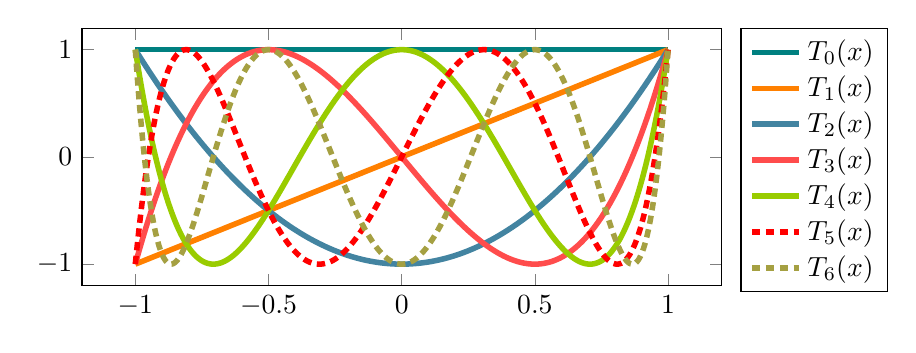
\begin{tikzpicture}
        \begin{axis}[domain=-1:1,legend pos=outer north east, samples=500, width=.8\linewidth, height=.4\linewidth,cycle list name=exotic]
            \addplot +[mark=none, line width=2pt] {cos(0*acos(x))};
            \addplot +[mark=none, line width=2pt] {cos(1*acos(x))};
            \addplot +[mark=none, line width=2pt] {cos(2*acos(x))};
            \addplot +[mark=none, line width=2pt] {cos(3*acos(x))};
            \addplot +[mark=none, line width=2pt] {cos(4*acos(x))};
            \addplot +[mark=none, line width=2pt] {cos(5*acos(x))};
            \addplot +[mark=none, line width=2pt] {cos(6*acos(x))};
            \legend{$T_{0}(x)$, $T_{1}(x)$, $T_{2}(x)$, $T_{3}(x)$, $T_{4}(x)$, $T_{5}(x)$, $T_6(x)$}
        \end{axis}
    \end{tikzpicture}
    \caption{Illustration of the first few Chebyshev polynomials over the interval $[-1, 1]$.}
    \label{fig:chebyshev}
\end{figure}

\begin{exercise}
    \label{exercise:chebychev}
    Show that~\eqref{eq:chebyshev} defines a polynomial of degree~$n$,
    and find its expression in the usual polynomial notation.
\end{exercise}
\begin{solution}
    The key idea is to rewrite the cosine function as the real part of a complex exponential:
    \[
        \cos (n \theta) = \Re \left( \e^{\i n \theta} \right)
            % = \Re \left( \left( \e^{\i \theta} \right)^n \right)
            = \Re \Bigl( \bigl( \cos (\theta) + \i \sin (\theta) \bigr)^n \Bigr).
    \]
    By expanding the power on the right-hand side,
    we can obtain an expression for $\cos(n \theta)$ in terms of $\cos(\theta)$ and $\sin(\theta)$.
    By the binomial formula,
    it holds that
    \[
        \bigl( \cos (\theta) + \i \sin (\theta) \bigr)^n
        = \sum_{j=0}^{n} \binom{n}{j} \cos(\theta)^{n-j}  \, \i^{j} \, \sin(\theta)^{j}.
    \]
    The terms corresponding to odd values of~$j$ are imaginary,
    and so these cancel out after taking the real part,
    which leads to
    \begin{align*}
        \cos (n \theta)
        &= \sum_{j=0}^{\lfloor n/2 \rfloor} \binom{n}{2j} \cos(\theta)^{n-2j}  \i^{2j} \sin(\theta)^{2j} \\
        &= \sum_{j=0}^{\lfloor n/2 \rfloor} (-1)^j \binom{n}{2j} \cos(\theta)^{n-2j}   \bigl(1 - \cos(\theta)^2\bigr)^j.
    \end{align*}
    Therefore,
    we conclude that
    \begin{equation}
        \label{eq:expression_chebyshev}
        T_n(x) = \sum_{j=0}^{\lfloor n/2 \rfloor} \binom{n}{2j} x^{n-2j}   \bigl(x - 1\bigr)^j.
    \end{equation}
\end{solution}

\begin{exercise}
    Show that the same polynomials are obtained from~\eqref{eq:chebyshev_cosh}.
\end{exercise}
\begin{solution}
    Notice that
    \begin{align*}
        \cosh(n \xi)
        &= \frac{1}{2} \left( \e^{n \xi} + \e^{-n \xi} \right) \\
        &= \frac{1}{2} \Bigl( \bigl(\cosh (\xi) + \sinh(\xi)\bigr)^n  + \bigl(\cosh(\xi) - \sinh(\xi)\bigr)^n \Bigr).
    \end{align*}
    Using the binomial formula, we obtain
    \begin{align*}
        \cosh(n \xi)
        &= \frac{1}{2}  \sum_{j=0}^{n} \binom{n}{j} \left( \cosh(\xi)^{n-j} \sinh(\xi)^j + \cosh(\xi)^{n-1} (-1)^j \sinh(\xi)^j \right) \\
        &=  \frac{1}{2} \sum_{j=0}^{n} \binom{n}{j} \cosh(\xi)^{n-j} \left( \sinh(\xi)^j + (-1)^j \sinh(\xi)^j \right).
    \end{align*}
    The contributions of the odd values of~$j$ cancel out,
    and so we obtain
    \begin{align*}
        \cosh(n \xi)
        &=  \sum_{j=0}^{\lfloor n / 2 \rfloor} \binom{n}{2j} \cosh(\xi)^{n-2j} \sinh(\xi)^{2j}.
    \end{align*}
    Since $\cosh(\xi)^2 - \sinh(\xi)^2 = 1$,
    we deduce that
    \[
        \cosh(n \xi)
        =  \sum_{j=0}^{\lfloor n / 2 \rfloor} \binom{n}{j} \cosh(\xi)^{n-2j} (\cosh(\xi)^2 - 1)^{j},
    \]
    which after the substitution of $\xi = \arccosh(x)$ leads to~\eqref{eq:expression_chebyshev}.
\end{solution}

\begin{exercise}
    [Recursion relation]
    \label{exercise:recursion_chebyshev}
    Show that the Chebyshev polynomials satisfy the relation
    \[
        \forall n \in \{2, 3, \dotsc\},
        \qquad
        T_{n+1} = 2 x T_{n} - T_{n-1}.
    \]
\end{exercise}
\begin{solution}
    It is sufficient to show the identity for $x \in [-1, 1]$,
    where the formula~\eqref{eq:chebyshev} applies.
    Using the well-known trigonometric identities,
    we have
    \begin{align*}
        \cos\bigl((n+1) \theta\bigr) &= \cos(n \theta) \cos(\theta) - \sin(n \theta) \sin (\theta)  \\
        \cos\bigl((n-1) \theta\bigr) &= \cos(n \theta) \cos(\theta) + \sin(n \theta) \sin (\theta).
    \end{align*}
    Adding both equations and rearranging, we obtain
    \[
        \cos\bigl((n+1) \theta\bigr) = 2 \cos(n \theta) \cos (\theta) - \cos\bigl((n-1) \theta\bigr).
    \]
    Therefore, using this equation with $\theta = \arccos(x)$,
    we obtain the statement.
\end{solution}

\begin{remark}
    The recursion relation in~\cref{exercise:recursion_chebyshev}
    can be employed to show by recursion that $T_n(x)$ is indeed a polynomial of degree~$n$.
\end{remark}

\begin{exercise}
    \label{exercise:chebyshev_leading_coefficient}
    Since $T_n\colon \real \to \real$ is a polynomial,
    it may be written in the standard form
    \[
        T_n(x) = \alpha^{(n)}_n x^n + \dotsc + \alpha^{(n)}_1 x + \alpha^{(n)}_0.
    \]
    Prove that~$\alpha^{(n)}_n = 2^{(n-1)}$ provided that $n \geq 1$.
\end{exercise}
\begin{solution}
    From the definition~\eqref{eq:chebyshev},
    the Chebychev polynomials of degrees 0 and 1 are given by $T_0(x) = 1$ and $T_1(x) = x$.
    The statement then follows by recursion, using~\cref{exercise:recursion_chebyshev}.
\end{solution}

It is immediate to show from~\eqref{eq:chebyshev} that the roots of $T_n$ are given by
\[
    x_k = \cos \left( \frac{\pi}{2n} + \frac{k\pi}{n} \right), \qquad k = 0, \dotsc, n-1.
\]
The polynomial $T_n$ takes the value 1 or -1 when evaluated at
\begin{equation}
    \label{eq:chebychev_maxima}
    z_k = \cos \left( \frac{k \pi}{n} \right), \qquad k = 0, \dotsc, n.
\end{equation}
More precisely, it holds that $T_n(z_k) = (-1)^k$.


\begin{exercise}
    Let $\xi \notin (-1, 1)$.
    Show that, among all the polynomials in $\poly(n)$ that are bounded from above by 1 in absolute value uniformly over the interval $(-1, 1)$,
    the Chebychev polynomial~$T_n$ achieves the largest absolute value when evaluated at~$\xi$.
\end{exercise}
\begin{solution}
    Reasoning by contradiction,
    we assume that $p$ satisfies
    \[
        \sup_{x \in (-1, 1)} \lvert p(x) \rvert \leq 1
    \]
    and $\lvert p(\xi) \rvert < \lvert T_n(\xi) \rvert$.
    Let $q(x) = p(x) T_n(\xi) / p(\xi)$.
    Then by construction $q(\xi) = T_n(\xi)$
    and
    \[
       \sup_{x \in (-1, 1)} \lvert q(x) \rvert < 1.
    \]
    Consequently, denoting by $z_k$ the points defined in~\eqref{eq:chebychev_maxima},
    we have that
    \[
        \forall k \in \{0, \dotsc, n\}, \qquad
        (-1)^k (T_n - q)(z_k) > 0.
    \]
    In other words, the polynomial $T_n - q$ takes positive values at $\{z_0, z_2, z_4, \dotsc\}$ and negative values at $\{z_1, z_3, z_5, \dotsc\}$.
    Consequently, by the intermediate value theorem,
    $T_n - q$ possesses~$n$ distinct roots in the open interval $(-1, 1)$.
    Since, in addition, $(T_n - q)(\xi) = 0$,
    we deduce that~$T_n - q$ has $n+1$ distinct roots,
    which is a contradiction given that $T_n - q$ is a nonzero polynomial of degree at most $n$.
\end{solution}
